

% sldies for T-61.6080 special course in bioinformatics 2, Spring 2015
\documentclass[first=dgreen,second=purple,logo=yellowexc]{aaltoslides}

% macro


% input encode
\usepackage[utf8]{inputenc}


%\usepackage[T1]{fontenc}
%\usepackage{lastpage}
%\usepackage{multirow}
%\usepackage{colortbl}
%\usepackage{comment}
%\usepackage{bm}
%\usepackage{natbib}


% Lipsum package generates bullshit
%\usepackage{lipsum}

% Set the document languages
%\usepackage[finnish,swedish,english]{babel}

% nomenclature
%\usepackage[intoc]{nomencl}

% math
\usepackage{amsmath}

% bibliograph
%\usepackage{natbib}

% For algorithms
\usepackage{algorithm}
\usepackage{algorithmic}

% math font
\usepackage{amsfonts}

% theory
%\usepackage{amsthm}

% double bracket
\usepackage{stmaryrd}

% special math symbol
\usepackage{amssymb}

% use enumerate environment
%\usepackage{enumitem}

% use \url \hyperref, make reference clickable
\usepackage{hyperref}

% use lastpage to inde
\usepackage{lastpage}



%-------------------
%
% set
%
%-------------------
\newcommand{\Acal}{\mathcal{A}}
\newcommand{\Bcal}{\mathcal{B}}
\newcommand{\Ccal}{\mathcal{C}}
\newcommand{\Dcal}{\mathcal{D}}
\newcommand{\Ecal}{\mathcal{E}}
\newcommand{\Fcal}{\mathcal{F}}
\newcommand{\Gcal}{\mathcal{G}}
\newcommand{\Hcal}{\mathcal{H}}
\newcommand{\Ical}{\mathcal{I}}
\newcommand{\Jcal}{\mathcal{J}}
\newcommand{\Kcal}{\mathcal{K}}
\newcommand{\Lcal}{\mathcal{L}}
\newcommand{\Mcal}{\mathcal{M}}
\newcommand{\Ncal}{\mathcal{N}}
\newcommand{\Ocal}{\mathcal{O}}
\newcommand{\Pcal}{\mathcal{P}}
\newcommand{\Qcal}{\mathcal{Q}}
\newcommand{\Rcal}{\mathcal{R}}
\newcommand{\Scal}{\mathcal{S}}
\newcommand{\Tcal}{\mathcal{T}}
\newcommand{\Ucal}{\mathcal{U}}
\newcommand{\Vcal}{\mathcal{V}}
\newcommand{\Wcal}{\mathcal{W}}
\newcommand{\Xcal}{\mathcal{X}}
\newcommand{\Ycal}{\mathcal{Y}}
\newcommand{\Zcal}{\mathcal{Z}}

\newcommand{\RR}{\mathbb{R}}
\newcommand{\ZZ}{\mathbb{Z}}

%-------------------
%
% vector
%
%-------------------
\newcommand{\va}{\mathbf {a}}
\newcommand{\vb}{\mathbf {b}}
\newcommand{\vc}{\mathbf {c}}
\newcommand{\vd}{\mathbf {d}}
\newcommand{\ve}{\mathbf {e}}
\newcommand{\vf}{\mathbf {f}}
\newcommand{\vg}{\mathbf {g}}
\newcommand{\vh}{\mathbf {h}}
\newcommand{\vi}{\mathbf {i}}
\newcommand{\vj}{\mathbf {j}}
\newcommand{\vk}{\mathbf {k}}
\newcommand{\vl}{\mathbf {l}}
\newcommand{\vm}{\mathbf {m}}
\newcommand{\vn}{\mathbf {n}}
\newcommand{\vo}{\mathbf {o}}
\newcommand{\vp}{\mathbf {p}}
\newcommand{\vq}{\mathbf {q}}
\newcommand{\vr}{\mathbf {r}}
\newcommand{\vs}{\mathbf {s}}
\newcommand{\vt}{\mathbf {t}}
\newcommand{\vu}{\mathbf {u}}
\newcommand{\vv}{\mathbf {v}}
\newcommand{\vw}{\mathbf {w}}
\newcommand{\vx}{\mathbf {x}}
\newcommand{\vy}{\mathbf {y}}
\newcommand{\vz}{\mathbf {z}}
\newcommand{\vmu}{\mathbf {\mu}}
\newcommand{\valpha}{\mathbf {\alpha}}
\newcommand{\vlambda}{\mathbf {\lambda}}
\newcommand{\vAlpha}{\mathbf {\Alpha}}
\newcommand{\vbeta}{\mathbf {\beta}}
\newcommand{\vBeta}{\mathbf {\Beta}}
\newcommand{\vgamma}{\mathbf {\gamma}}
\newcommand{\vGamma}{\mathbf {\Gamma}}
\newcommand{\vdelta}{\mathbf {\dalta}}
\newcommand{\vDelta}{\mathbf {\Dalta}}
\newcommand{\vone}{\mathbf {1}}
\newcommand{\vzero}{\mathbf {0}}
\newcommand{\vell}{\mathbf {\ell}}
\newcommand{\vxi}{\mathbf{\xi}}
\newcommand{\vphi}{\mathbf{\phi}}
\newcommand{\vPhi}{\mathbf{\Phi}}

%-------------------
%
% math operation
%
%-------------------
\newcommand{\argmax}{\textbf{argmax}}
\newcommand{\argmin}{\textbf{argmin}}
\newcommand{\sign}{\textbf{sign}}
\newcommand{\maximize}{\textbf{max}}
\newcommand{\minimize}{\textbf{min}}
\newcommand{\argkmax}{\textbf{argkmax}}
\newcommand{\argkmin}{\textbf{argkmin}}
\newcommand{\kmaximize}{\textbf{kmax}}
\newcommand{\kminimize}{\textbf{kmin}}
\newcommand{\st}{\textbf{s.t.}}
\newcommand{\set}[1]{\{ #1 \}}
%\newcommand{\ind}[1]{{\llbracket #1 \rrbracket}}
\newcommand{\ind}[1]{\mathbf{1}_{\{#1\}}}
\newcommand{\norm}[1]{\left|\left| #1 \right|\right|}
\newcommand{\ip}[2]{\langle #1, #2 \rangle}
\newcommand{\var}{\textbf{Var}}
\newcommand{\E}{\textbf{E}}
\newcommand{\exponential}[1]{e^{ #1 }}


\newcommand{\Gva}{G_{\va}}
%-------------------
%
% writings
%
%-------------------
\newcommand{\eqdef}{\overset{{\rm \mbox{\tiny def}}}{=}}
\newcommand{\sbf}[1]{\boldsymbol{#1}}
\newcommand{\mbf}[1]{\mathbf{#1}} 
\newcommand{\etal}{{\em et al.}}

\newcommand{\svmstruct}{{\sc ssvm}}
\newcommand{\mmmn}{{\sc m$^3$n}}
\newcommand{\svm}{{\sc svm}}
\newcommand{\mmcrf}{{\sc mmcrf}}
\newcommand{\smo}{{\sc smo}}
\newcommand{\crf}{{\sc crf}}
\newcommand{\nphard}{$\Ncal\Pcal$-hard}
\newcommand{\nphardness}{$\Ncal\Pcal$-hardness}
\newcommand{\iis}{{\sc iis}}
\newcommand{\memm}{{\sc memm}}
\newcommand{\lr}{{\sc lr}}
\newcommand{\svmlight}{{\sc svmlight}}
\newcommand{\libsvm}{{\sc libsvm}}
\newcommand{\svmcascade}{{\sc svmcascade}}
\newcommand{\adaboost}{{\sc adaboost}}
\newcommand{\adaboostmh}{{\sc adaboost.mh}}
\newcommand{\bagging}{{\sc bagging}}
\newcommand{\vrtree}{{\sc vr-tree}}
\newcommand{\deepboosting}{{\sc deepboosting}}
\newcommand{\loo}{{\sc loo}}
\newcommand{\mtl}{{\sc mtl}}
\newcommand{\sdp}{{\sc sdp}}
\newcommand{\iqp}{{\sc iqp}}
\newcommand{\qp}{{\sc qp}}
\newcommand{\daggraph}{{\sc dag}}
\newcommand{\lp}{{\sc lp}}

\newcommand{\hatf}{{\hat{f}}}
\newcommand{\p}{\sc p}
\newcommand{\n}{\sc n}
\newcommand{\pp}{\sc pp}
\newcommand{\pn}{\sc pn}
\newcommand{\nn}{\sc nn}
\newcommand{\maxcut}{{\sc max-cut}}
\newcommand{\greedy}{{\sc greedy}}
\newcommand{\kernelcascade}{{\sc kernel cascade}}
\newcommand{\netrate}{{\sc netrate}}
\newcommand{\netinf}{{\sc netinf}}
\newcommand{\spin}{{\sc spin}}
\newcommand{\vI}{\mathbf{I}}
\newcommand{\tp}{^{\intercal}}
\newcommand{\mve}{{\sc mve}}
\newcommand{\amm}{{\sc amm}}
\newcommand{\mam}{{\sc mam}}
\newcommand{\rta}{{\sc rta}}
\newcommand{\lasso}{{\sc lasso}}
\newcommand{\mle}{{\sc mle}}
\newcommand{\map}{{\sc map}}
\newcommand{\rbf}{{\sc rbf}}
\newcommand{\mlknn}{{\sc ml-knn}}
\newcommand{\knn}{{\sc knn}}
\newcommand{\iblr}{{\sc iblr}}
\newcommand{\cc}{{\sc cc}}
\newcommand{\pcc}{{\sc pcc}}
\newcommand{\ecc}{{\sc ecc}}
\newcommand{\br}{{\sc br}}
\newcommand{\corrlog}{{\sc corrlog}}
\newcommand{\ilgs}{{\sc ilgs}}
\newcommand{\ilrs}{{\sc ilrs}}
\newcommand{\cpp}{{\sc c}}
\newcommand{\matlab}{{\sc matlab}}
\newcommand{\openmp}{{\sc openmp}}
\newcommand{\python}{{\sc python}}
\newcommand{\cvx}{{\sc cvx}}
\newcommand{\lda}{{\sc lda}}
\newcommand{\kkt}{{\sc k.k.t}}
\newcommand{\lbp}{{\sc lbp}}
\newcommand{\anova}{{\sc anova}}

\renewcommand{\algorithmicrequire}{\textbf{Input:}}
\renewcommand{\algorithmicensure}{\textbf{Output:}}



\newcommand{\Upsilonb}{\pmb \Upsilon}
\newcommand{\phib}{\pmb \phi}
\newcommand{\psib}{\pmb \psi}
\newcommand{\varphib}{\pmb \varphi}
\newcommand{\phibh}{\hat\phib}
\newcommand{\psibh}{\hat \psib}
\newcommand{\vYcal}{\pmb \Ycal}
\newcommand{\vXcal}{\pmb \Xcal}
\newcommand{\vFcal}{\pmb \Fcal}
%-------------------
%
% others
%
%-------------------




%\newtheorem{definition}{Definition}
%\newtheorem{theory}{Theory}
%\newtheorem{lemma}{Lemma}














% title and other informtions
\title{Multilabel classification through structured output learning}
\subtitle{Multilabel classification}
\author[H. Su]{Hongyu Su}
\institute[ICS]{Department of Computer Science\\School of Science, Aalto University\\hongyu.su@aalto.fi}
\aaltofootertext{Molecular classification}{\today}{\arabic{page}/\pageref{LastPage}\ }

%\date{Version 1.0, \today}
\date{ \today}
\AtBeginSection[]
{
  \begin{frame}<beamer>{Outline}
    \tableofcontents[currentsection,subsection]
  \end{frame}
}


% start the main contain of the document
\begin{document}


\aaltotitleframe



\footnotesize{

\begin{frame}{Example: dog vs. cat?}
	\begin{itemize}
		\item We have $5000$ pictures of dog and $5000$ pictures of cat.
		\begin{center}
			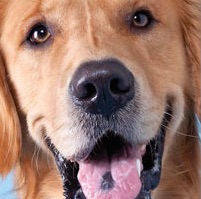
\includegraphics[scale=0.3]{./figures/dog.jpg}
			\text{     }
			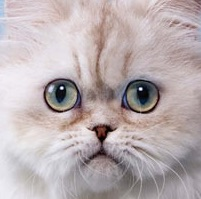
\includegraphics[scale=0.3]{./figures/cat.jpg}
		\end{center}
		\item Computer digitalize each picture into $100\times100$ pixels.
		\item Given a new picture, we want to answer: is it a dog or a cat?
		\item Simple task for human, dog, or cat.
		\item \citet{Golle08machine} claimed this is a difficult task for machines with only $82.7\%$ accuracy.
		\item In 2013, $98.5\%$ accuracy was reported in a Kaggle competition (https://www.kaggle.com/c/dogs-vs-cats).
	\end{itemize}
\end{frame}

\begin{frame}{In human verification system}
	\begin{itemize}
		\item Human verification system is a program that protects website from robots by generating and grading test that human can pass but machine cannot.
		\item CAPTCHA system \citep{Ahn03captcha} uses distorted text.
		\begin{center}
			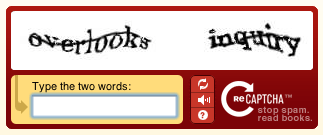
\includegraphics[scale=0.2]{./figures/captcha.png}
		\end{center}
		\item ASIRRA system \citep{Elson07asirra} uses images.
		\begin{center}
			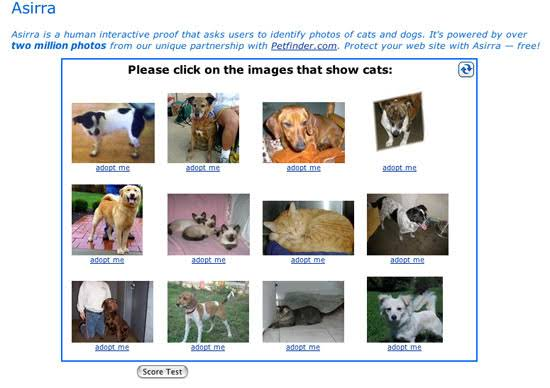
\includegraphics[scale=0.2]{./figures/assira.jpg}
		\end{center}
		\item To test if the ASIRRA system is safe from machine learning attack.
		\begin{itemize}
			\footnotesize
			\item One should get all $12$ pictures right!
			\item Accuracy for machine is $(98.5\%)^{12} \approx 83.4\%$.
		\end{itemize}
	\end{itemize}
\end{frame}

\begin{frame}{In search engine}
	\begin{itemize}
		\item If machine can assign cat/dog to all pictures correctly, we can search pictures with keywords.
		\only<1>{\item Search all \textbf{cat} pictures.}
		\only<2>{\item Search all \textbf{dog} pictures.}
	\end{itemize}
	\only<1>{
	\begin{center}
		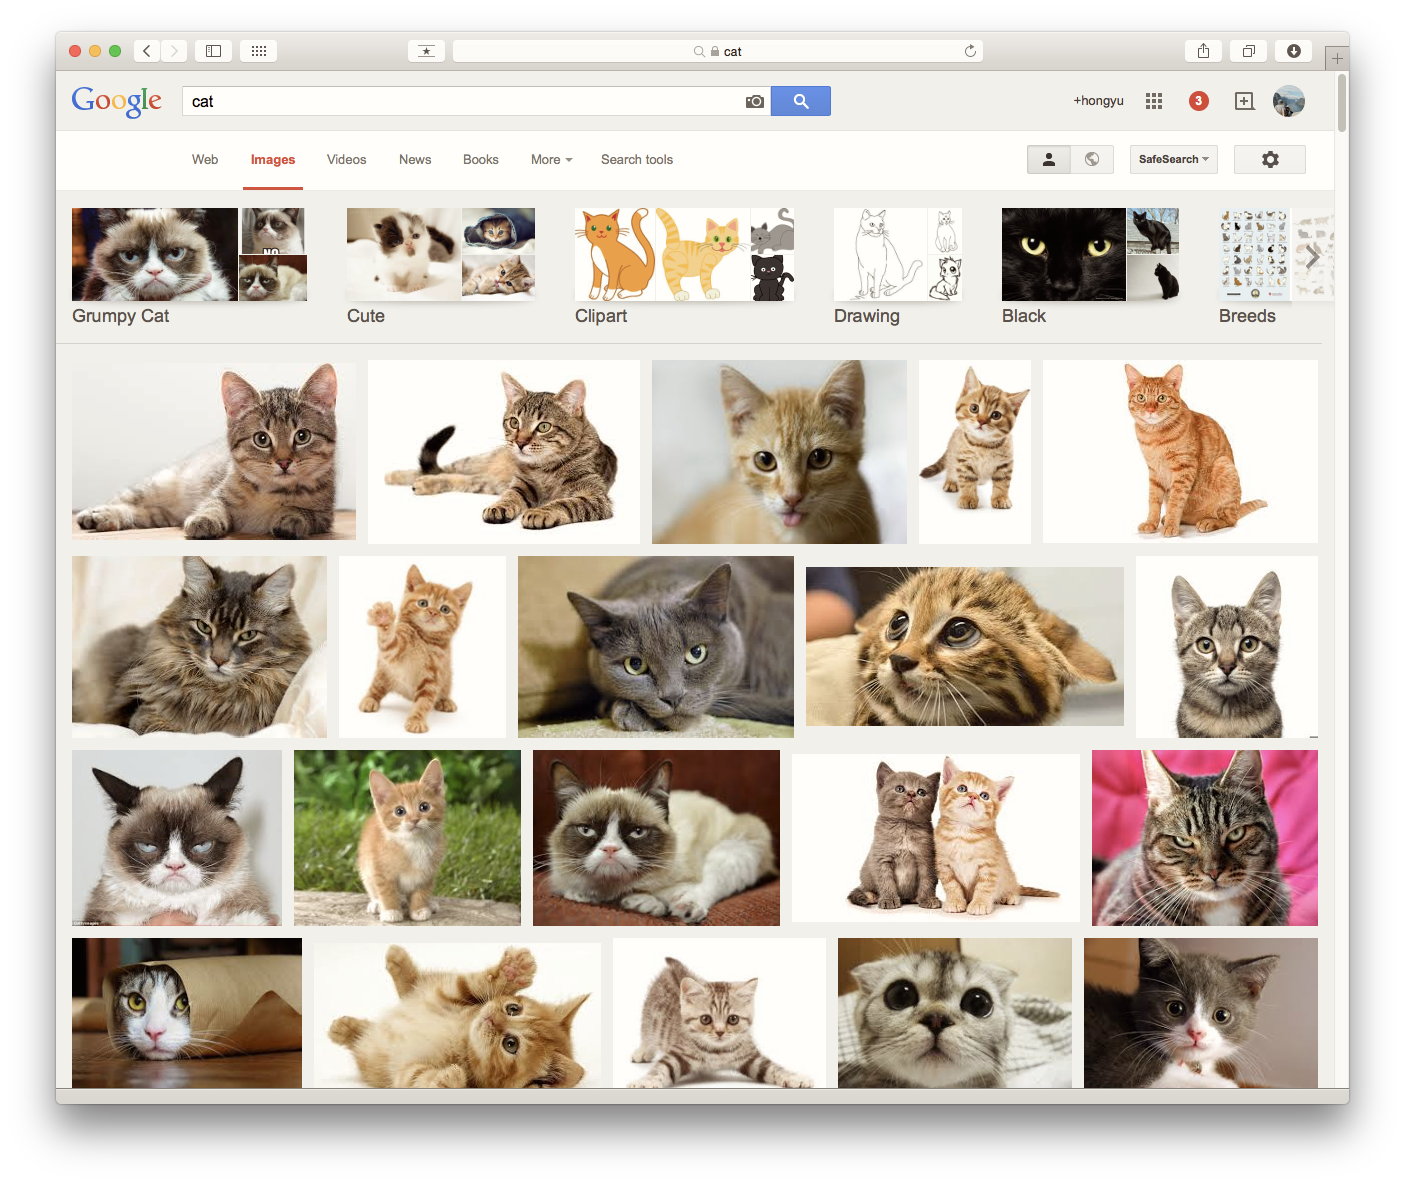
\includegraphics[scale=0.13]{./figures/googlecat.png}
	\end{center}
	}
	\only<2>{
	\begin{center}
		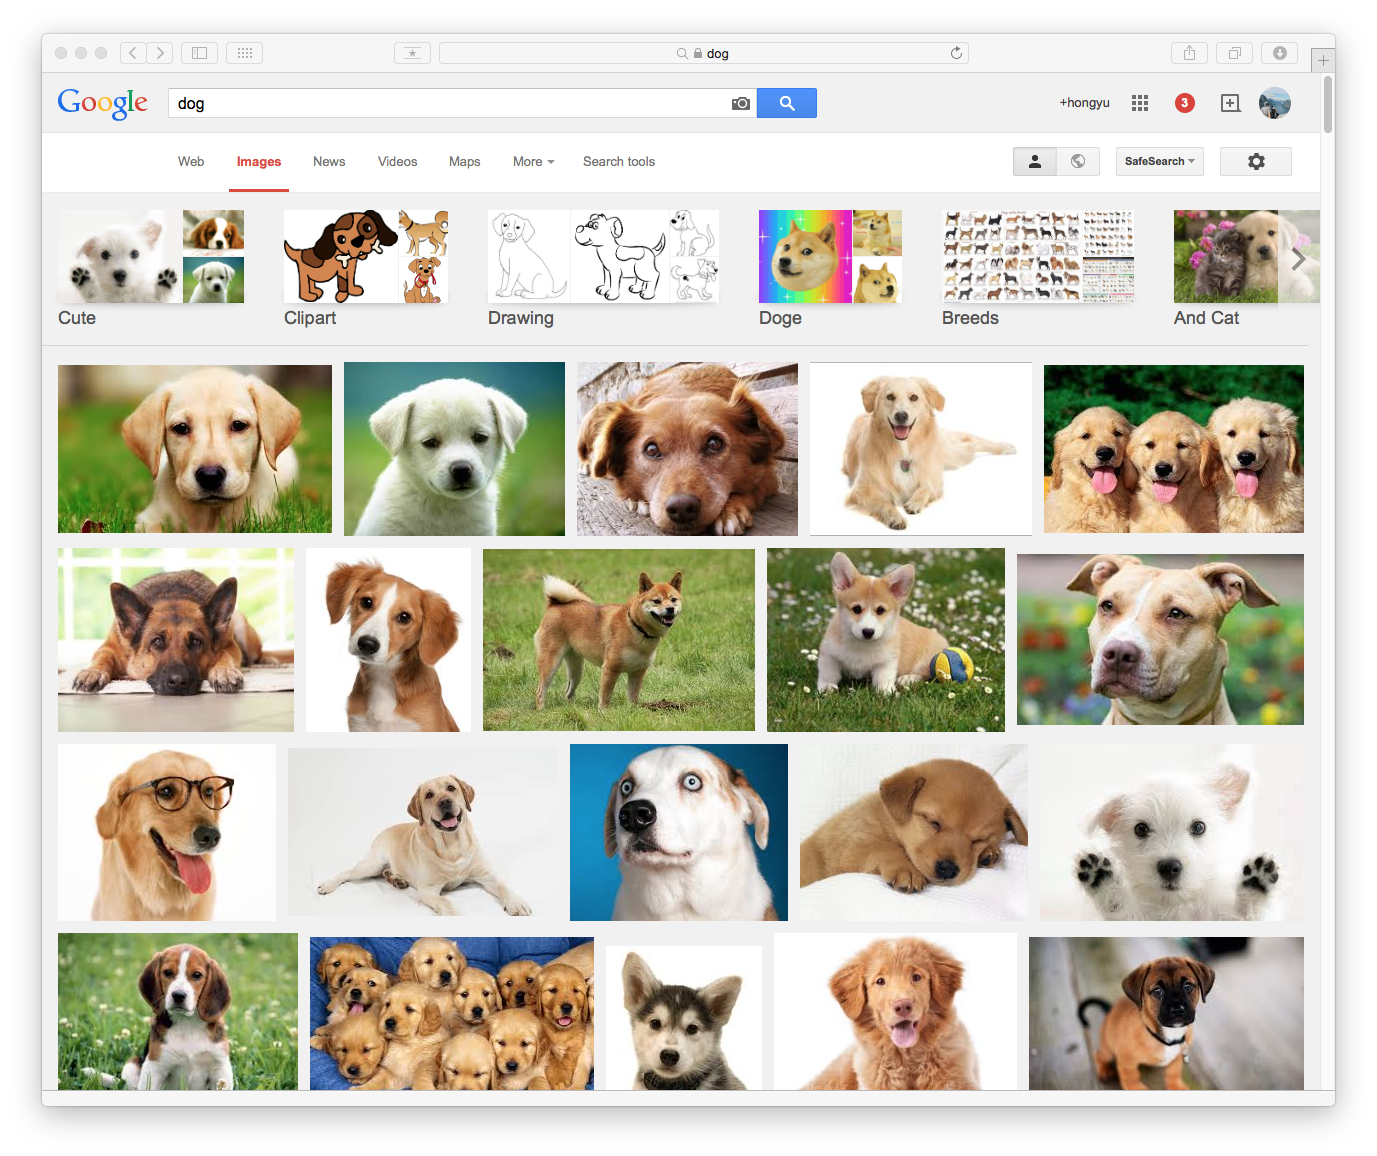
\includegraphics[scale=0.13]{./figures/googledog.png}
	\end{center}
	}
\end{frame}


\begin{frame}{Single label classification}
	\begin{itemize}
		\item In machine learning, the problem is known as \textit{single label classification}.
		\begin{itemize}
			\footnotesize
			\item Input is an object $\vx$ (e.g., an image).
			\item Output is an attribute $y$ called \textit{label} (e.g., $y=+1$:dog, $y=-1$:cat).
			\item Explore a set of known object and label pairs called \textit{training data} \\
			(e.g., $\{(\vx_1,+1),\cdots,(\vx_{5001},-1),\cdots\}$).
			\item Learn a \textit{mapping function} that predicts the label of a new object.
			\begin{align*}
				\vx\overset{f}{\rightarrow}y,y\in\{+1,-1\}.
			\end{align*}
		\end{itemize}
		\item Many algorithms are available to tackle single label classification problems, e.g., support vector machines \citep{Cortes95support}, logistic regression \citep{Chen99}.
	\end{itemize}
\end{frame}

\iffalse
\item Mathematically, we define the single label classification problem
\begin{itemize}
	\footnotesize
	\item Data come in pairs $(\vx,y)\in\vXcal\times\Ycal$, sampled from some unknown distribution $P(\vx.y)$.
	\item $\vXcal=\RR^d$ is a domain of input, $\Ycal=\{+1,-1\}$ is a domain of output.
	\item We are given a set of training data $\Scal=\{(\vx_i,y_i)\}_{i=1}^{m}$.
	\item Learn a mapping function $f\in\Hcal$ that predict the best output of an input
	\begin{align*}
		\vx\overset{f}{\rightarrow}y
	\end{align*}
\end{itemize}
\fi


\begin{frame}{Image annotation task}
	\begin{itemize}
		\item We are interested in multiple attributes (labels) of a single image.
		\item For example, we want to annotate all images with multiple labels \\
		\{boat, sea, sun, beach, people, dog, cat\}
		\item Correct annotations will allow us to search with multiple attributes.
		\only<1>{\item Search with \textbf{boat \& sea \& sun}}.
		\only<2>{\item Search with \textbf{sun \& beach \& people}}.
		\only<3>{\item Search with \textbf{dog \& cat}}.
	\end{itemize}
	\only<1>{
	\begin{center}
		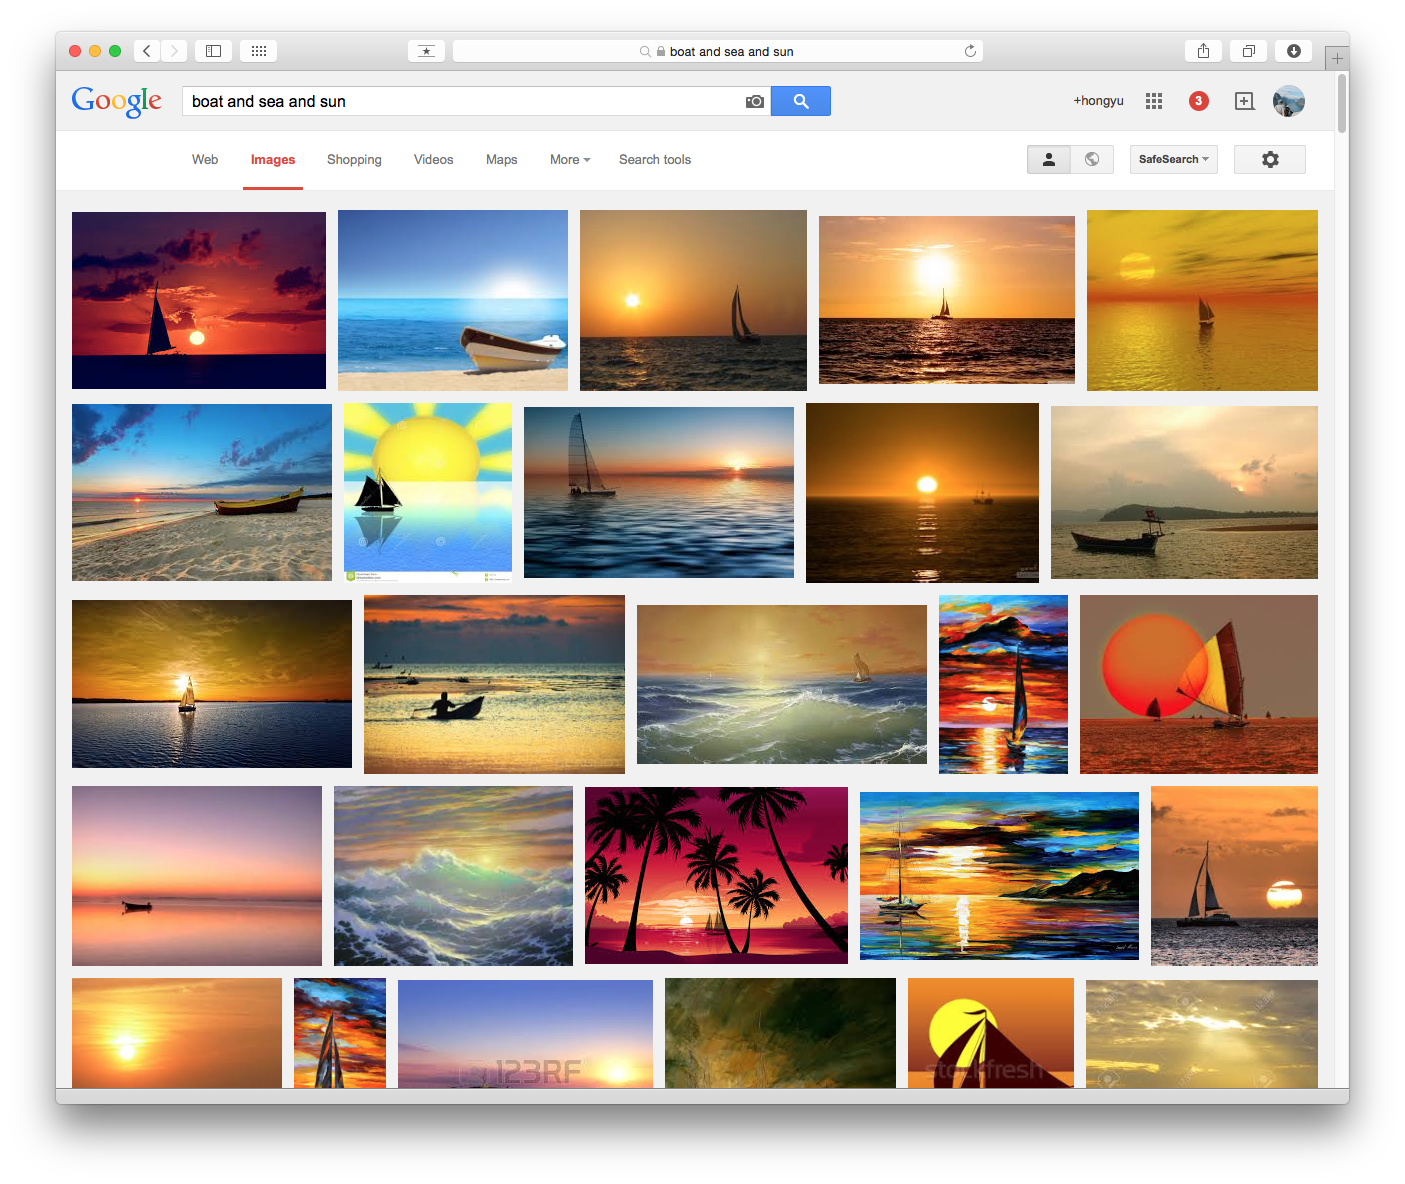
\includegraphics[scale=0.11]{./figures/googleboat.png}
	\end{center}
	}
	\only<2>{
	\begin{center}
		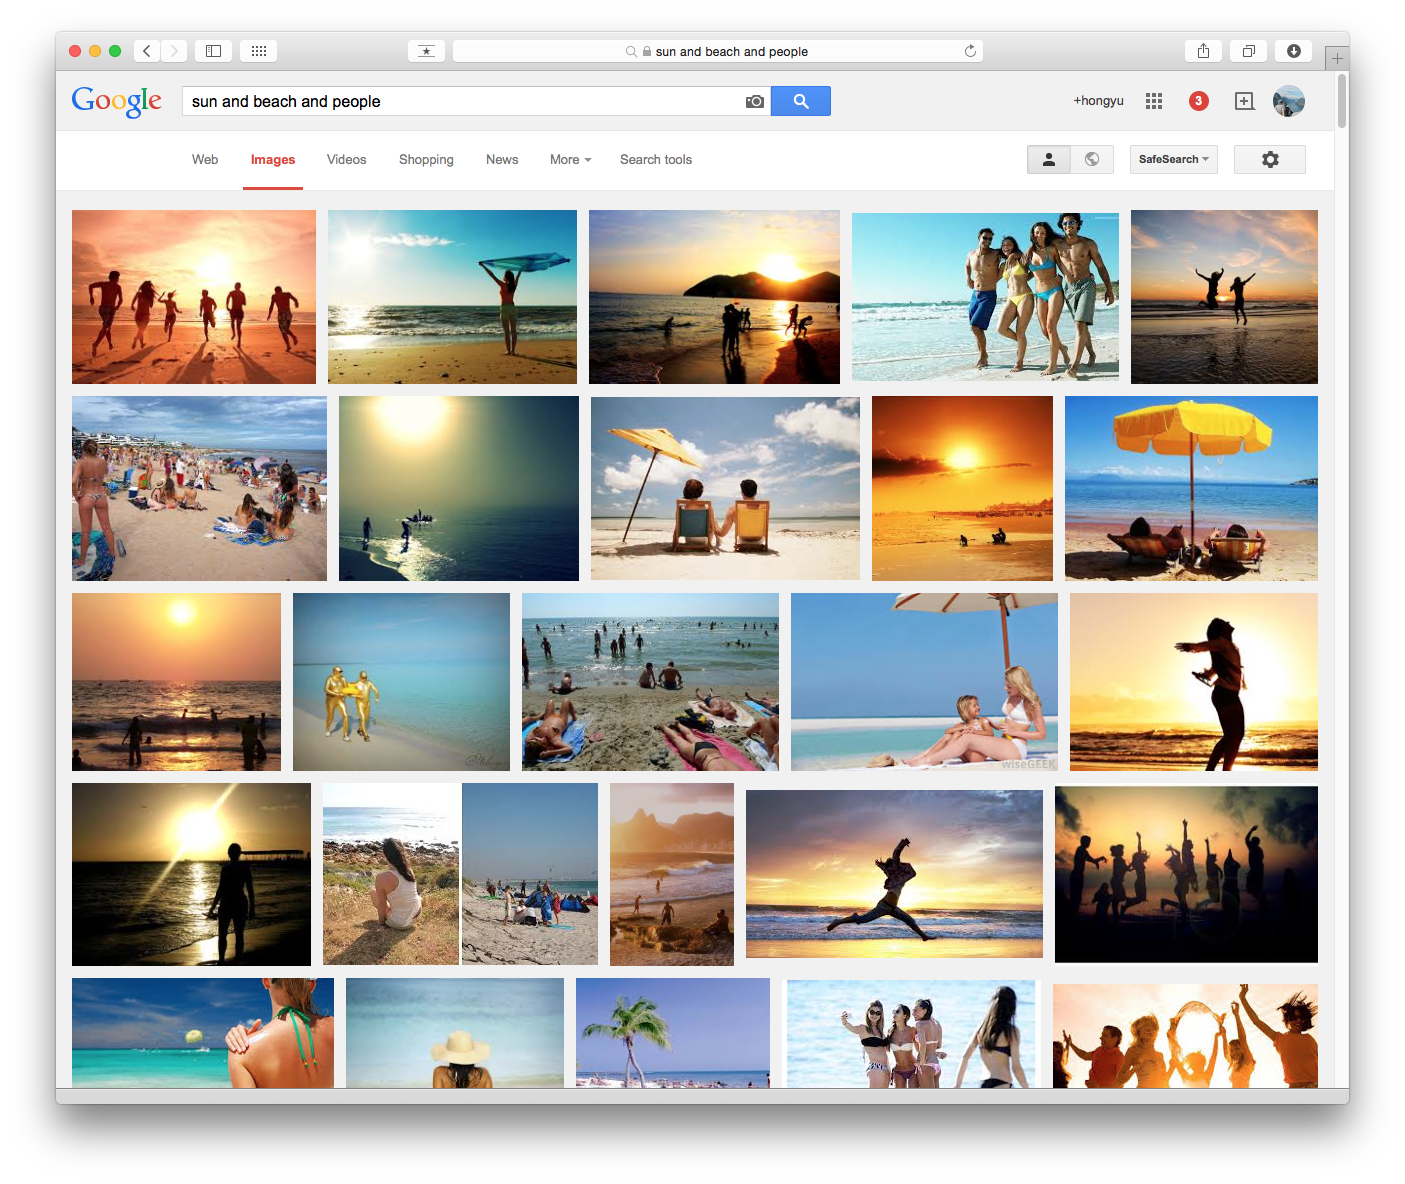
\includegraphics[scale=0.11]{./figures/googlesun.png}
	\end{center}
	}
	\only<3>{
	\begin{center}
		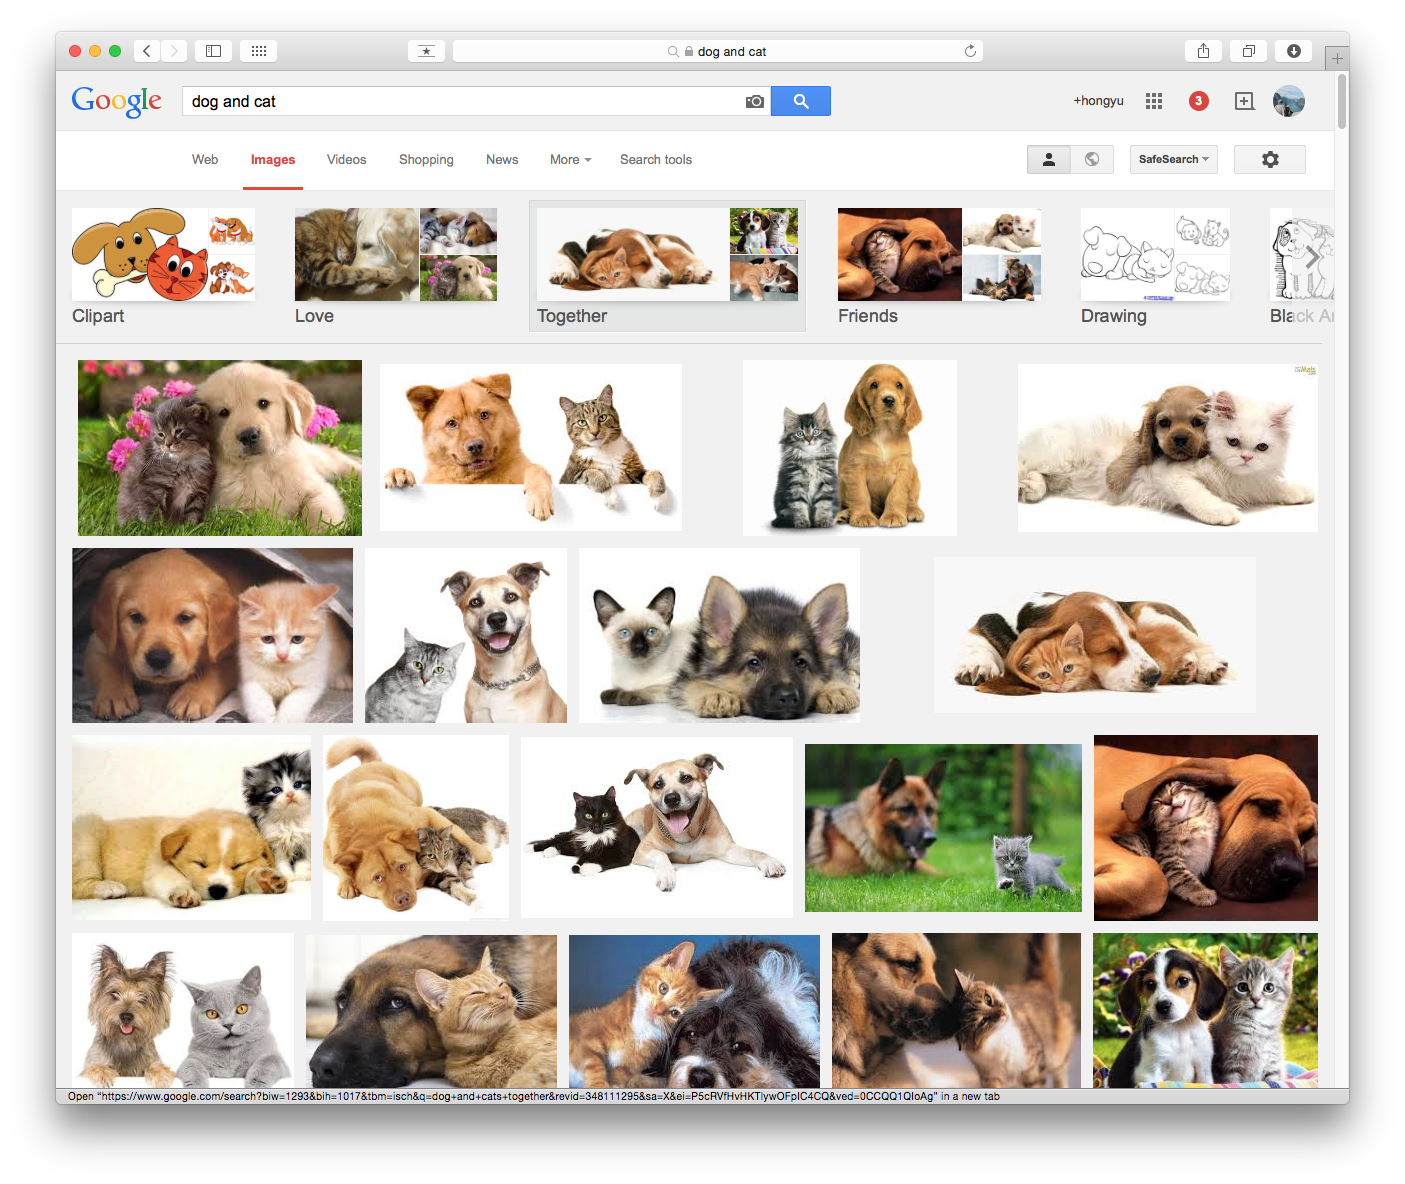
\includegraphics[scale=0.11]{./figures/googledogcat.png}
	\end{center}
	}
\end{frame}


\begin{frame}{Multilabel classification}
	\begin{itemize}
		\item The problem is known as \textit{multilabel classification}, which is a natural extension to single label classification.
		\begin{itemize}
			\footnotesize
			\item Input is an object $\vx$ (e.g., an image).
			\item Output are multiple attributes $\vy$ called \textit{multilabel}\\
			(e.g., $\vy=(\underbrace{+1}_{\text{boat}},\underbrace{+1}_{\text{sea}},\underbrace{-1}_{\text{sun}},\underbrace{-1}_{\text{beach}},\underbrace{+1}_{\text{people}},\underbrace{-1}_{\text{dog}},\underbrace{-1}_{\text{cat}})$).
			\item Explore a set of known object and label pairs called {training data} \\
			\item Learn a \textit{mapping function} that predicts the best multilabel of a new object.
			\begin{align*}
				\vx\overset{f}{\rightarrow}\vy=(y_1,\cdots,y_k).
			\end{align*}
		\end{itemize}
		\item Multilabel classification is an active research field in machine learning.
	\end{itemize}
\end{frame}

\begin{frame}{Applications}
	\begin{itemize}
		\item Image annotation is to annotate an image with multiple tags.
		\begin{tabular}{p{3cm}p{10cm}}
        \multirow{2}{*}{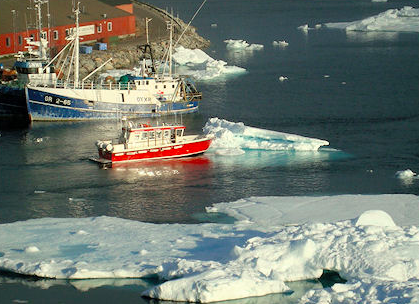
\includegraphics[scale = 0.13]{./figures/boatsea.png}} & \\
		& $(\underbrace{+1}_{\text{boat}},\underbrace{+1}_{\text{sea}},\underbrace{-1}_{\text{sun}},\underbrace{-1}_{\text{beach}},\underbrace{-1}_{\text{people}},\underbrace{+1}_{\text{ice}},\underbrace{+1}_{\text{land}})$\\
        \end{tabular}
		\item Document classification is to classify a document into multiple categories.\\
		\begin{tabular}{p{3cm}p{10cm}} 
        \multirow{2}{*}{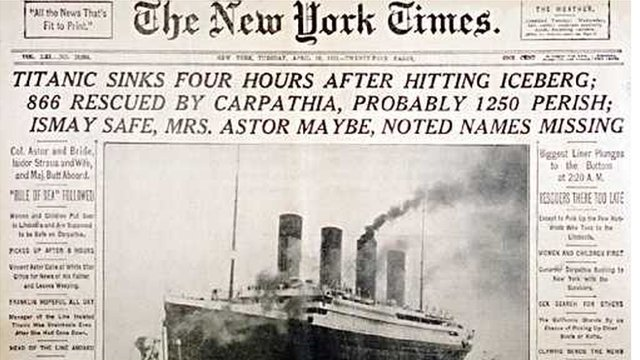
\includegraphics[scale = 0.13]{./figures/titanic.jpg}} & \\
		& $(\underbrace{+1}_{\text{news}},\underbrace{+1}_{\text{economics}},\underbrace{-1}_{\text{sports}},\underbrace{-1}_{\text{politics}},\underbrace{-1}_{\text{movie}},\underbrace{-1}_{\text{science}},\underbrace{-1}_{\text{art}})$\\
        \end{tabular}
		\item Molecular classification is to predict drug activities in different targets.\\
		\begin{tabular}{p{3cm}p{10cm}} 
        \multirow{2}{*}{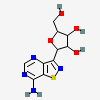
\includegraphics[scale = 0.4]{./figures/mol1.png}} & \\
		& $(\underbrace{+1}_{\text{target1}},\underbrace{-1}_{\text{target2}},\underbrace{-1}_{\text{target3}},\underbrace{-1}_{\text{target4}},\underbrace{-1}_{\text{target5}},\underbrace{+1}_{\text{target6}},\underbrace{+1}_{\text{target7}})$\\
        \end{tabular}
		\item Social network analysis is to predict how a message spreads.
		\begin{tabular}{p{3cm}p{10cm}} 
        \multirow{2}{*}{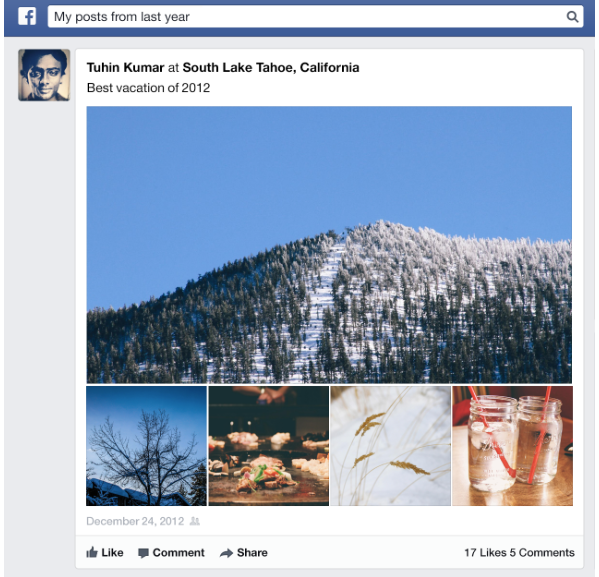
\includegraphics[scale = 0.08]{./figures/facebookvideo.png}} & \\
		& $(\underbrace{+1}_{\text{Ted}},\underbrace{-1}_{\text{Alice}},\underbrace{+1}_{\text{David}},\underbrace{-1}_{\text{Mark}},\underbrace{+1}_{\text{Alex}},\underbrace{-1}_{\text{Zoe}},\underbrace{-1}_{\text{Frank}})$\\
        \end{tabular}
	\end{itemize}
\end{frame}


\begin{frame}{How to solve multilabel classification?}
	\begin{itemize}
		\item Reduce the multilabel classification problem as a collection of single label classification problems.
		\item Solve each individual problem independently. 
		\item Combine the results.
	\end{itemize}
	\only<1>{
	\begin{tabular}{p{1.5cm}p{0.5cm}p{3cm}} 
    \multirow{2}{*}{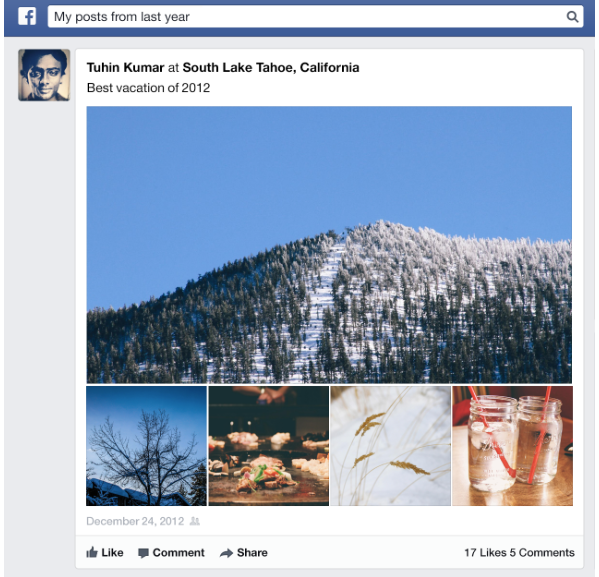
\includegraphics[scale = 0.08]{./figures/facebookvideo.png}} & &\\
	& $\overset{f}{\rightarrow}$ &$(\underbrace{?}_{\text{Ted}},\underbrace{?}_{\text{Alice}},\underbrace{?}_{\text{David}},\underbrace{?}_{\text{Mark}},\underbrace{?}_{\text{Alex}},\underbrace{?}_{\text{Zoe}},\underbrace{?}_{\text{Frank}})$\\
    \end{tabular}
	}
	\only<2>{
	\begin{tabular}{p{1.5cm}p{0.5cm}p{3cm}} 
    \multirow{2}{*}{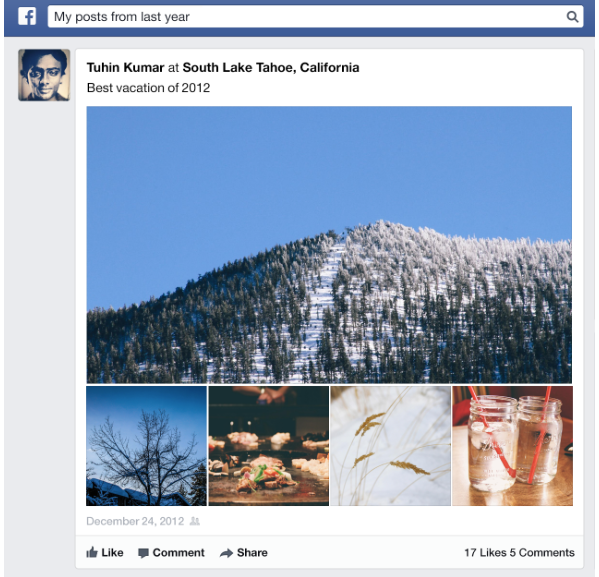
\includegraphics[scale = 0.08]{./figures/facebookvideo.png}} & &\\
	& $\overset{f_1}{\rightarrow}$ &$(\underbrace{+1}_{\text{Ted}},\underbrace{}_{\text{Alice}},\underbrace{}_{\text{David}},\underbrace{}_{\text{Mark}},\underbrace{}_{\text{Alex}},\underbrace{}_{\text{Zoe}},\underbrace{}_{\text{Frank}})$\\
    \end{tabular}
	}
	\only<3>{
	\begin{tabular}{p{1.5cm}p{0.5cm}p{3cm}} 
    \multirow{2}{*}{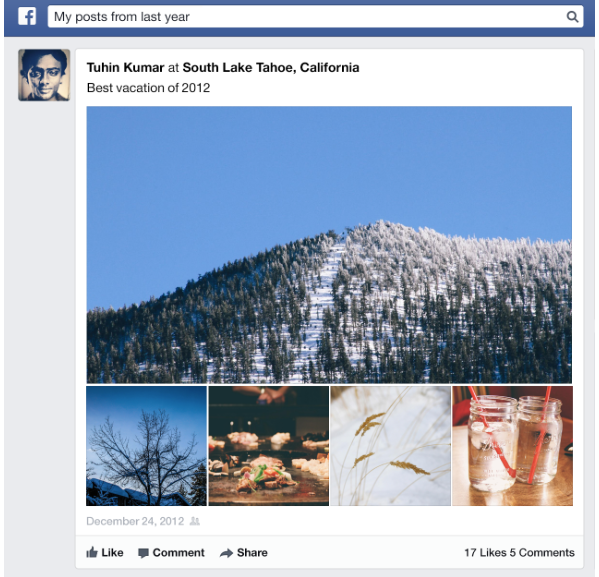
\includegraphics[scale = 0.08]{./figures/facebookvideo.png}} &  &\\
	& $\overset{f_2}{\rightarrow}$ &$(\underbrace{}_{\text{Ted}},\underbrace{-1}_{\text{Alice}},\underbrace{}_{\text{David}},\underbrace{}_{\text{Mark}},\underbrace{}_{\text{Alex}},\underbrace{}_{\text{Zoe}},\underbrace{}_{\text{Frank}})$\\
    \end{tabular}
	}
	\only<4>{
	\begin{tabular}{p{1.5cm}p{0.5cm}p{3cm}} 
    \multirow{2}{*}{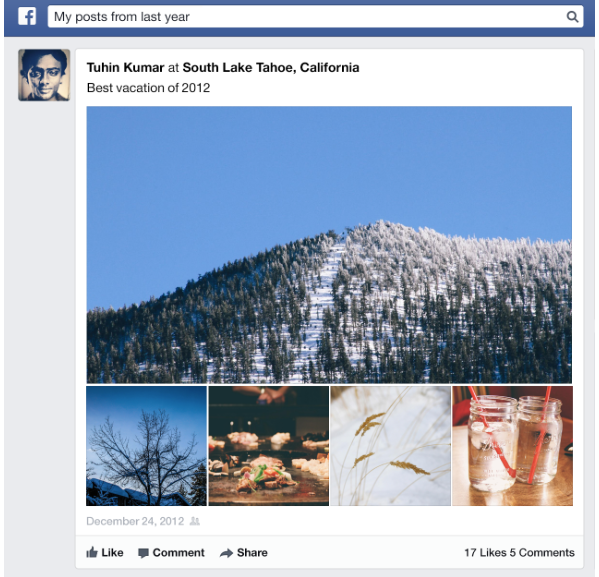
\includegraphics[scale = 0.08]{./figures/facebookvideo.png}} &  &\\
	& $\overset{f_3}{\rightarrow}$ &$(\underbrace{}_{\text{Ted}},\underbrace{}_{\text{Alice}},\underbrace{+1}_{\text{David}},\underbrace{}_{\text{Mark}},\underbrace{}_{\text{Alex}},\underbrace{}_{\text{Zoe}},\underbrace{}_{\text{Frank}})$\\
    \end{tabular}
	}
	\only<5>{
	\begin{tabular}{p{1.5cm}p{0.5cm}p{3cm}} 
    \multirow{2}{*}{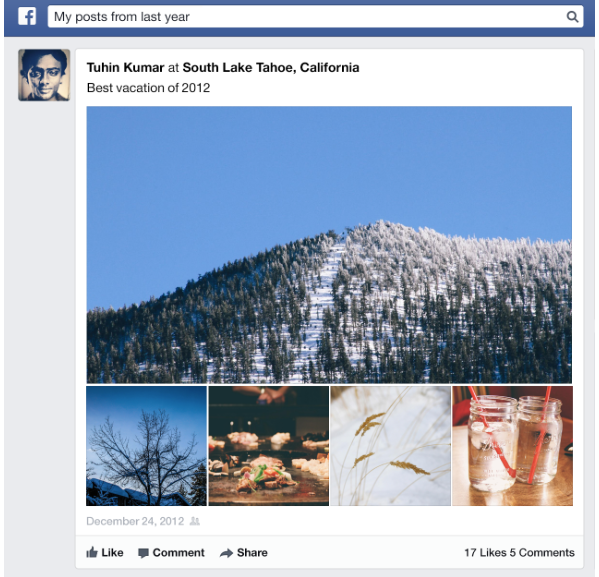
\includegraphics[scale = 0.08]{./figures/facebookvideo.png}} &  &\\
	& $\overset{f_4}{\rightarrow}$ &$(\underbrace{}_{\text{Ted}},\underbrace{}_{\text{Alice}},\underbrace{}_{\text{David}},\underbrace{-1}_{\text{Mark}},\underbrace{}_{\text{Alex}},\underbrace{}_{\text{Zoe}},\underbrace{}_{\text{Frank}})$\\
    \end{tabular}
	}
	\only<6>{
	\begin{tabular}{p{1.5cm}p{0.5cm}p{3cm}} 
    \multirow{2}{*}{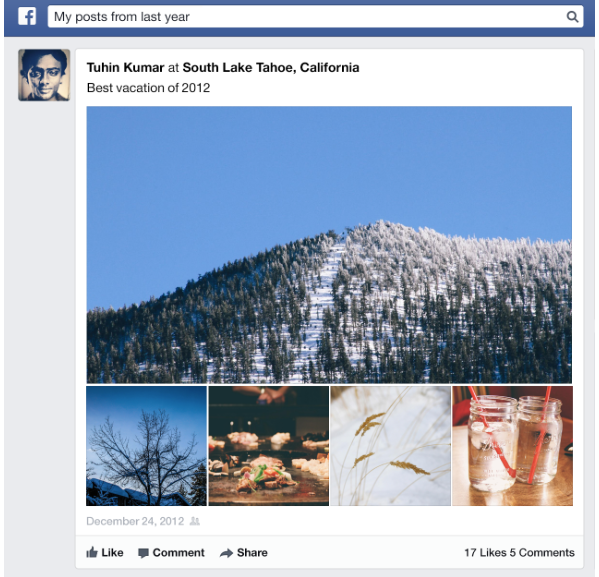
\includegraphics[scale = 0.08]{./figures/facebookvideo.png}} &  &\\
	& $\overset{f_1,\cdots,f_7}{\rightarrow}$ &$(\underbrace{+1}_{\text{Ted}},\underbrace{-1}_{\text{Alice}},\underbrace{+1}_{\text{David}},\underbrace{-1}_{\text{Mark}},\underbrace{+1}_{\text{Alex}},\underbrace{-1}_{\text{Zoe}},\underbrace{-1}_{\text{Frank}})$\\
    \end{tabular}
	}
	
	
	
\end{frame}


\begin{frame}{Label correlations}
	\begin{itemize}
		\item Multiple attributes are closely related. Similar attributes will have similar response to an input.
		\begin{itemize}
			\item Social network analysis: friends have similar hobbies.
			\begin{align*}
		(\underbrace{+1}_{\text{Ted}},\underbrace{-1}_{\text{Alice}},\underbrace{+1}_{\text{David}},\underbrace{-1}_{\text{Mark}},\underbrace{+1}_{\text{Alex}},\underbrace{-1}_{\text{Zoe}},\underbrace{-1}_{\text{Frank}})
			\end{align*}
			\begin{center}
				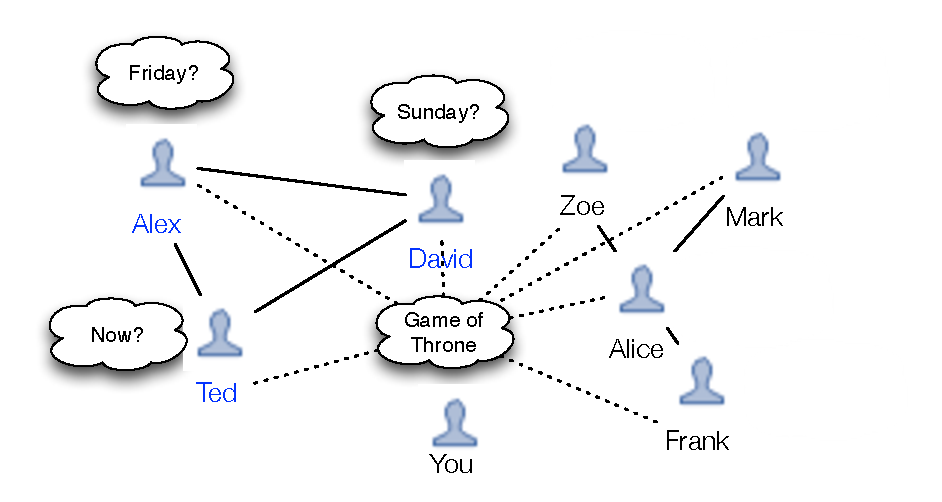
\includegraphics[scale=0.5]{./figures/facebooknetwork.pdf}
			\end{center}
			\item Document classification: A news about movies ma
	\end{itemize}
	\end{itemize}
\end{frame}



\begin{frame}{To get benefit?}
	\begin{itemize}
		\item Fingerprint identification
		\item Voice recognition
		\item Information assistant
	\end{itemize}
\end{frame}


\begin{frame}{To contribute?}
	\begin{itemize}
		\item SETI@home
		\item Rosetta@home
		\item Foldit
	\end{itemize}
\end{frame}










\begin{frame}[allowframebreaks]{Bibliography}
%\bibliographystyle{plain}
\bibliographystyle{apalike}
 \bibliography{dissertation}
\end{frame}

}
\end{document}
%%%%%%%%%%%%%%%%%%%%%%%%%%%%%%%%%%%%%%%%%%%%%%%%%%%%%%%%%%%%%%%%%%%%%%%%%%%%%%%%%%%%%%%%%%%%%






